\documentclass[aspectratio=169,11pt]{beamer}
\usepackage[utf8]{inputenc}
\usepackage[french]{babel}
\usepackage[T1]{fontenc}
\usepackage{graphicx}
\usepackage{tikz}
\usetikzlibrary{shapes,arrows,positioning,shadows,calc}
\usepackage{booktabs}
\usepackage{xcolor}
\usetheme{Madrid}
\definecolor{primarycolor}{RGB}{37,99,235}
\definecolor{secondarycolor}{RGB}{71,85,105}
\definecolor{successcolor}{RGB}{16,185,129}
\definecolor{warningcolor}{RGB}{245,158,11}
\definecolor{dangercolor}{RGB}{239,68,68}
\setbeamercolor{palette primary}{bg=primarycolor,fg=white}
\setbeamercolor{structure}{fg=primarycolor}
\setbeamercolor{frametitle}{bg=primarycolor,fg=white}
\setbeamertemplate{navigation symbols}{}
\setbeamertemplate{footline}[frame number]

\title[Audit de biais COMPAS]{\LARGE\bfseries Audit de biais d'un modèle de classification}
\subtitle{Étude du dataset COMPAS ProPublica}
\institute{Filière Intelligence Artificielle et Cybersécurité}
\author{\textbf{Réalisé par :} À renseigner\\\textbf{Encadré par :} À renseigner}
\date{\today}
\titlegraphic{\IfFileExists{ensabm.png}{\includegraphics[height=1.5cm]{ensabm.png}}{}}

\begin{document}
\begin{frame}[plain]\titlepage\end{frame}
\begin{frame}{Sommaire}\tableofcontents\end{frame}

\section{Contexte}
\begin{frame}{Problématique}
\begin{block}{Question centrale}
Le modèle prend-il des décisions équitables entre groupes sensibles, et comment réduire les disparités sans détruire la performance ?
\end{block}
\begin{itemize}
\item Cas réel : prédiction de récidive à deux ans.
\item Attributs audités : \texttt{race} et \texttt{sex}.
\item Risque majeur : faux positifs différenciés selon les groupes.
\end{itemize}
\end{frame}

\begin{frame}{Dataset COMPAS}
\begin{itemize}
\item Source : ProPublica, \texttt{compas-scores-two-years.csv}.
\item Cible : \texttt{two\_year\_recid}.
\item Variables : âge, antécédents, type d'accusation, score COMPAS.
\item Limite : les labels judiciaires ne sont pas une vérité sociale neutre.
\end{itemize}
\end{frame}

\section{Méthodologie}
\begin{frame}{Pipeline expérimental}
\begin{enumerate}
\item Nettoyage COMPAS et EDA orientée biais.
\item Split train/validation/test stratifié.
\item Baselines : Logistic Regression, Random Forest, MLP.
\item Audit : DP, DI, EO, TPR/FPR, selection rate.
\item Mitigation : reweighting, resampling, Fairlearn, PyTorch adversarial, seuils.
\end{enumerate}
\end{frame}

\begin{frame}{Pourquoi garder les attributs sensibles ?}
\begin{alertblock}{Point critique}
Retirer \texttt{race} ou \texttt{sex} des features ne prouve pas l'absence de biais : d'autres variables peuvent agir comme proxys.
\end{alertblock}
\end{frame}

\section{Résultats}
\begin{frame}{Performance baseline}
\begin{center}
\begin{tabular}{lr}
\toprule
Métrique & Valeur \\
\midrule
Accuracy & 0.692 \\
F1-score & 0.625 \\
ROC-AUC & 0.751 \\
Baseline & \texttt{logistic\_regression} \\
\bottomrule
\end{tabular}
\end{center}
\end{frame}

\begin{frame}{Fairness baseline}
\begin{center}
\begin{tabular}{lrr}
\toprule
Attribut & EO diff & DP diff \\
\midrule
race & 0.652 & 0.495 \\
sex & 0.117 & 0.131 \\
\bottomrule
\end{tabular}
\end{center}
\end{frame}

\begin{frame}{Visualisations}
\IfFileExists{../reports/figures/eda_demographics.png}{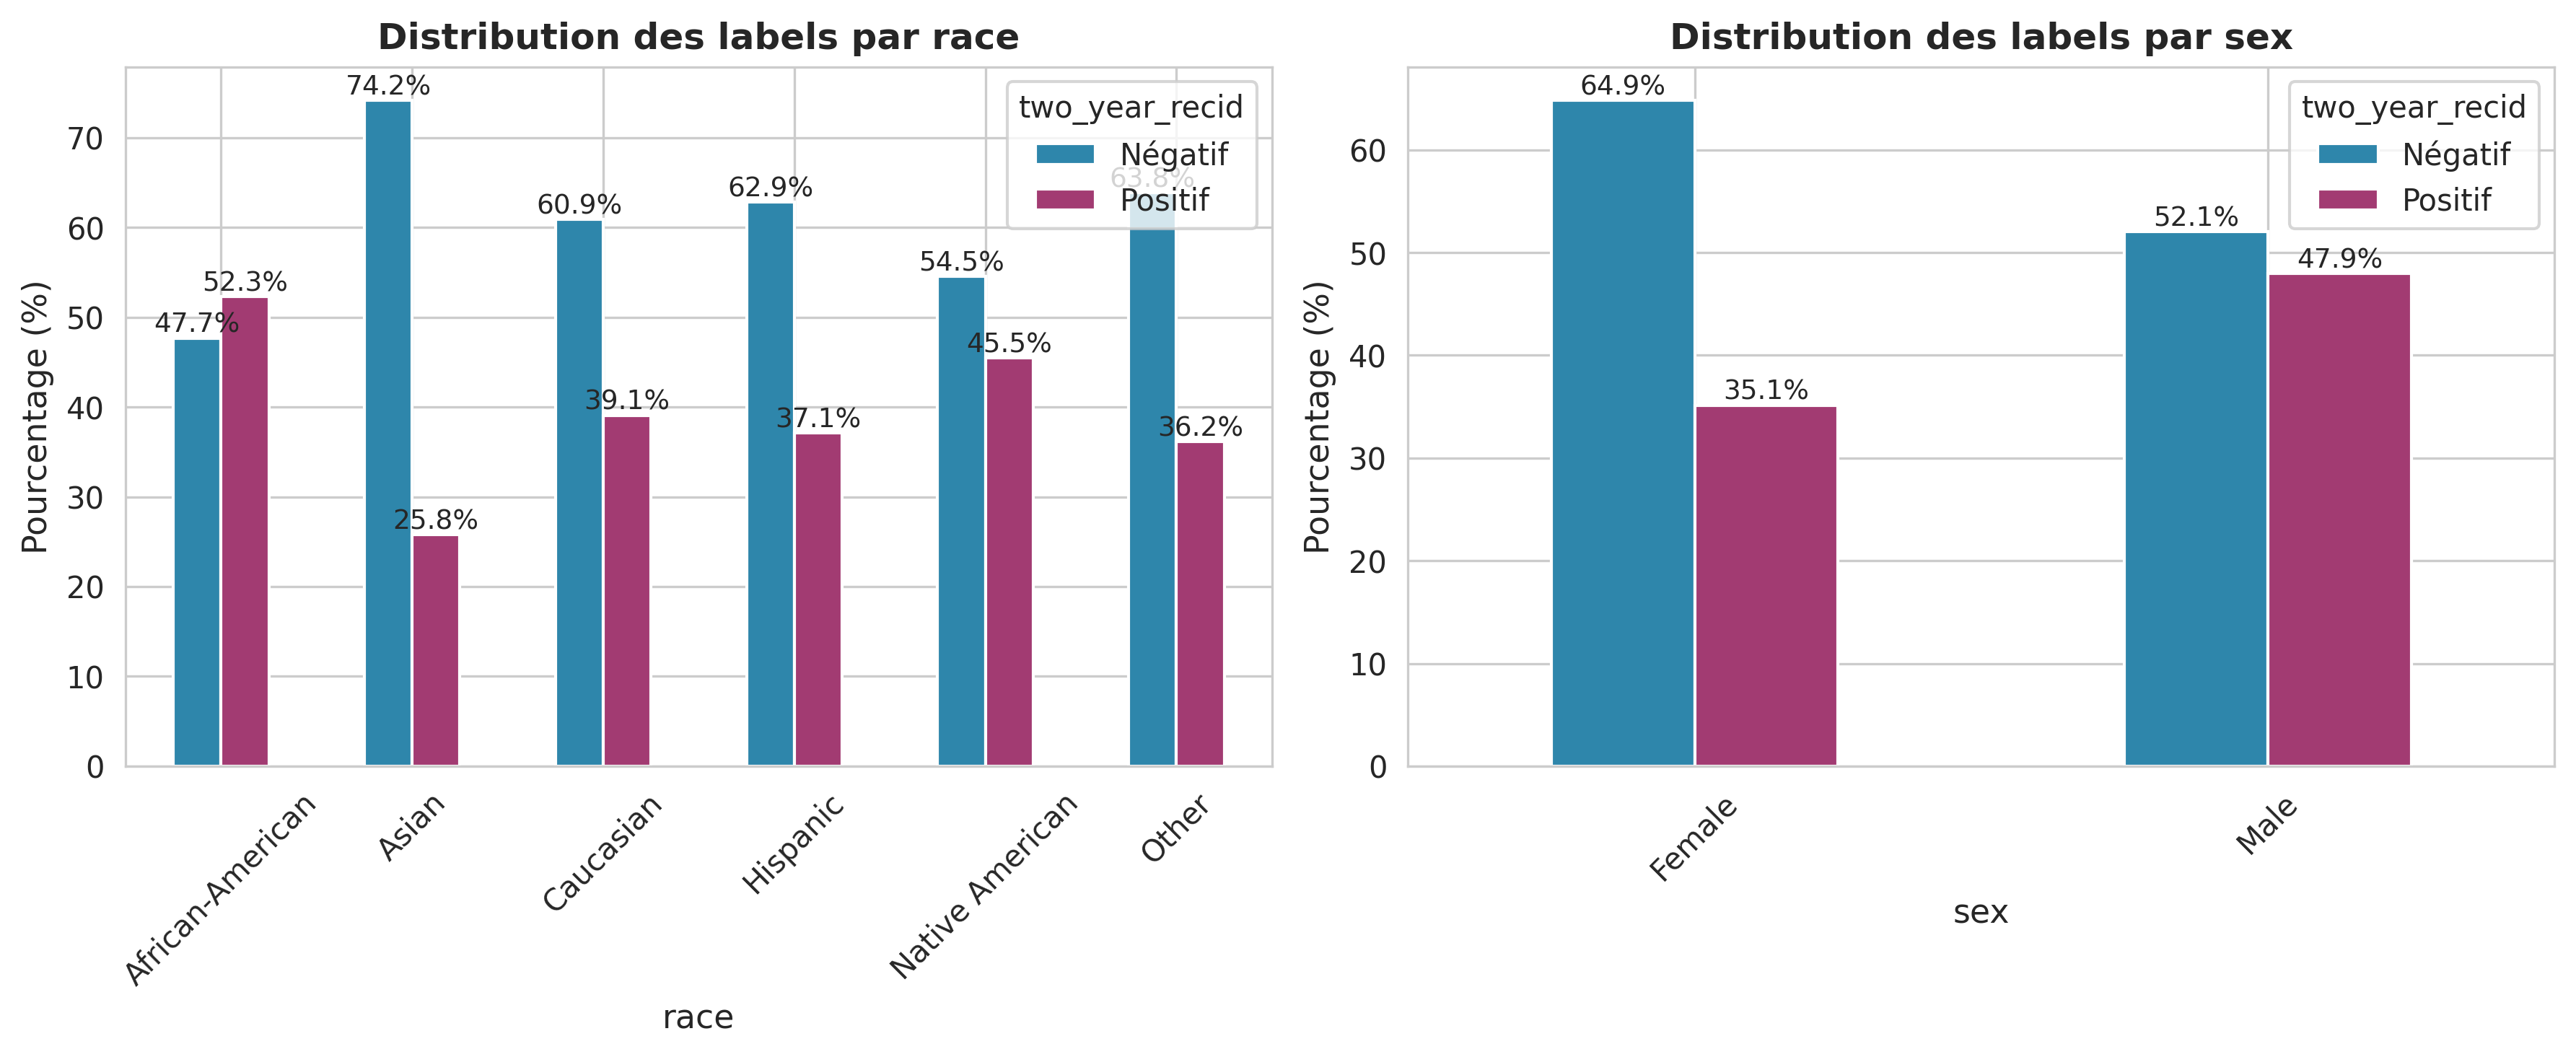
\includegraphics[width=.48\textwidth]{../reports/figures/eda_demographics.png}}{}
\IfFileExists{../reports/figures/debiasing_comparison.png}{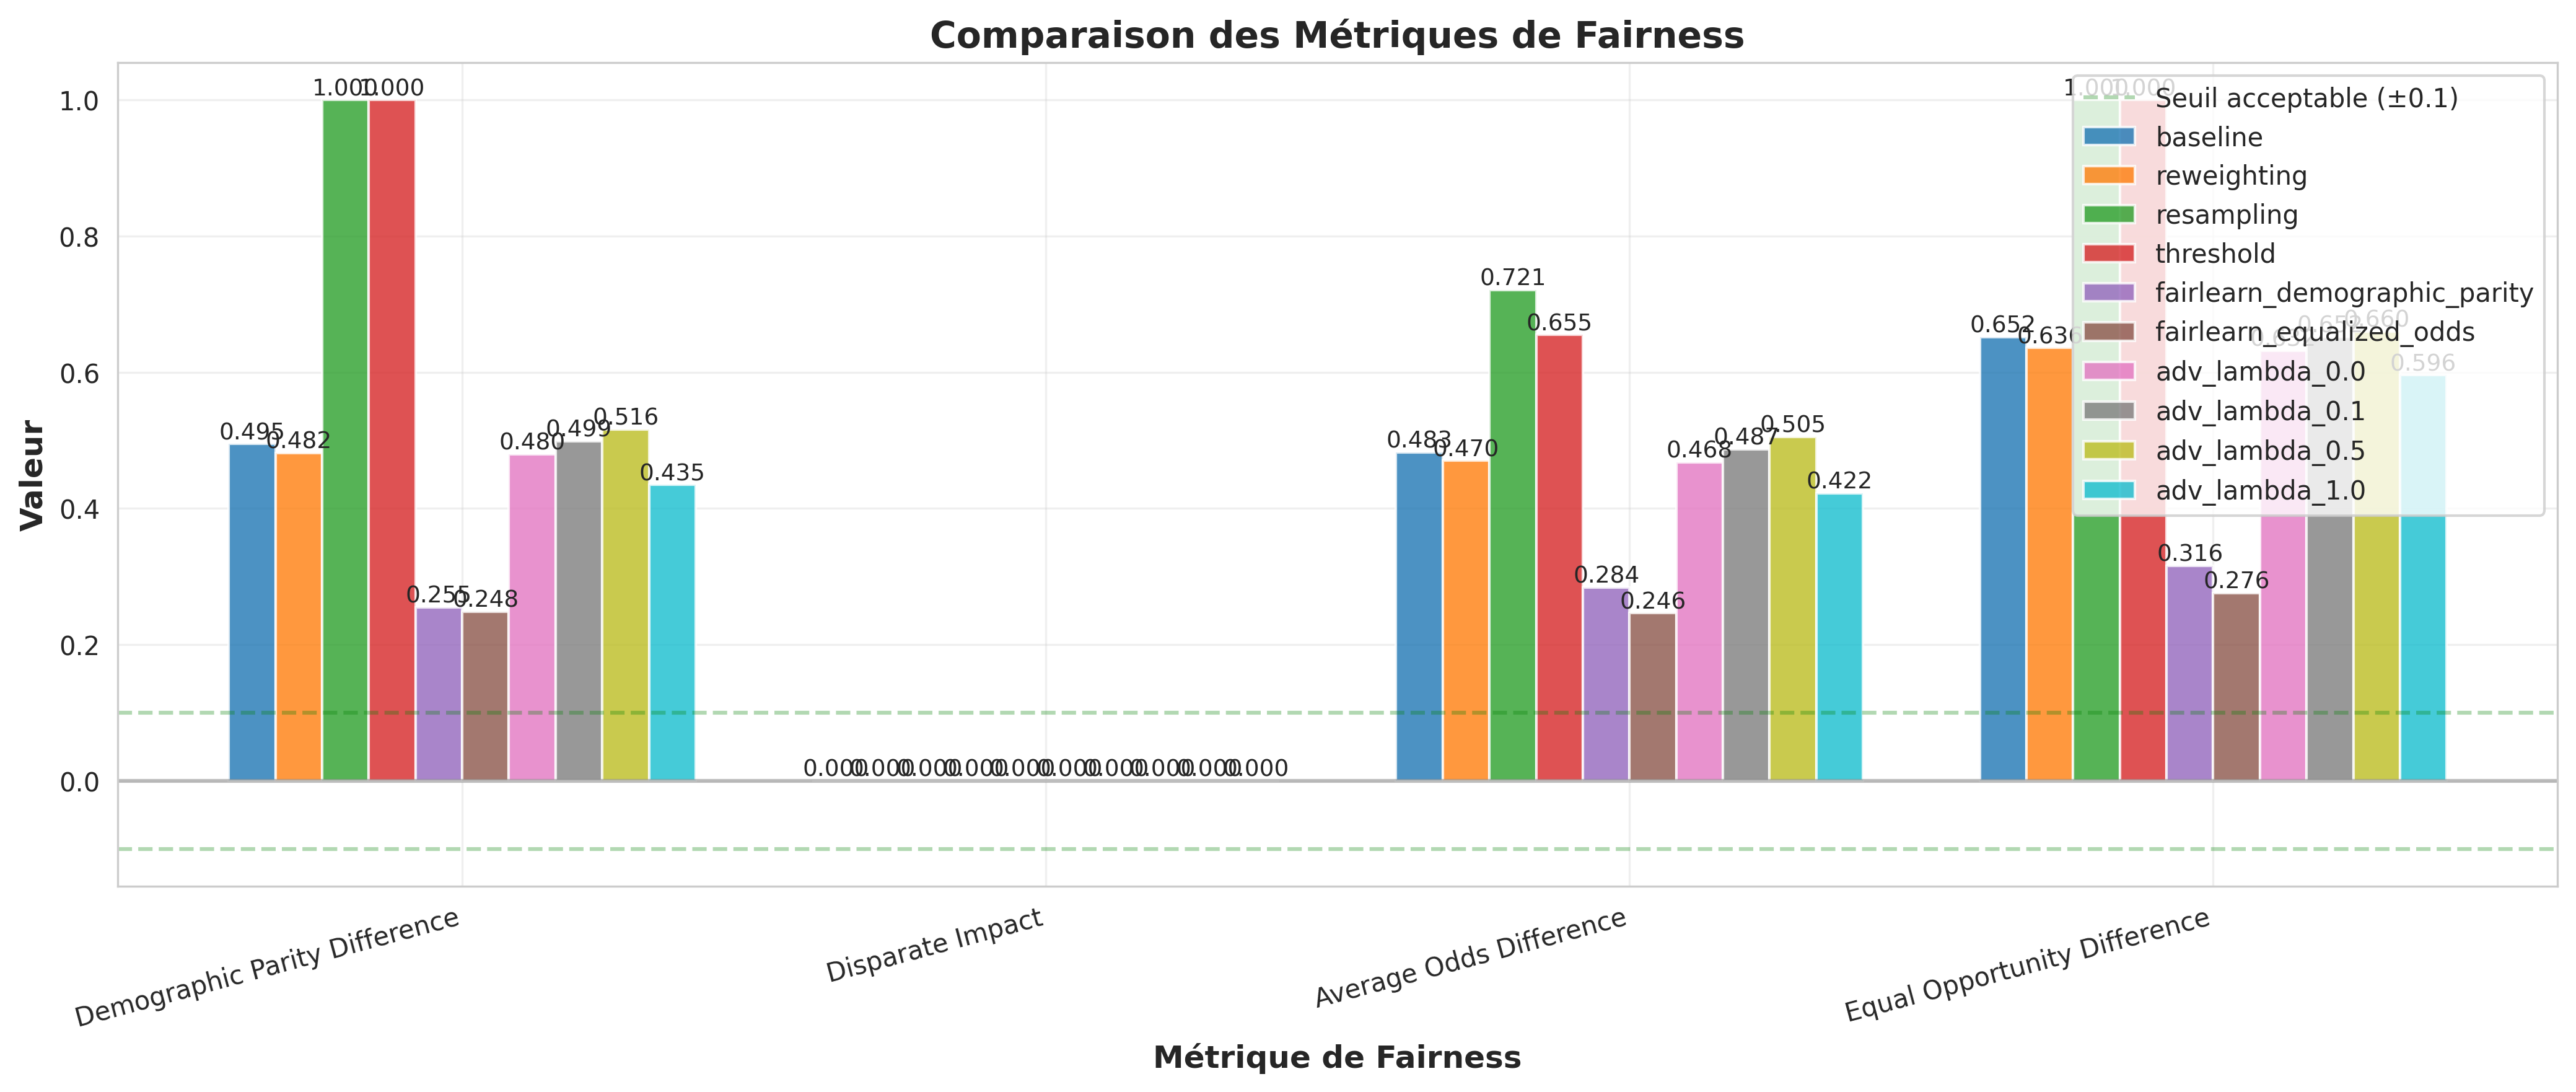
\includegraphics[width=.48\textwidth]{../reports/figures/debiasing_comparison.png}}{}
\end{frame}

\section{Mitigation}
\begin{frame}{Méthodes comparées}
\begin{itemize}
\item \textbf{Reweighting} : pondération par couples groupe/label.
\item \textbf{Resampling} : équilibrage des sous-groupes.
\item \textbf{Fairlearn} : contraintes demographic parity/equalized odds.
\item \textbf{Adversarial PyTorch} : représentation moins informative sur l'attribut sensible.
\item \textbf{Post-processing} : seuils par groupe, à discuter éthiquement.
\end{itemize}
\end{frame}

\begin{frame}{Recommandations}
\begin{itemize}
\item Ne jamais se limiter à l'accuracy globale.
\item Auditer systématiquement TPR/FPR par groupe.
\item Privilégier equalized odds pour les erreurs en contexte judiciaire.
\item Documenter les limites COMPAS et surveiller la dérive après déploiement.
\end{itemize}
\end{frame}

\section{Conclusion}
\begin{frame}{Conclusion}
\begin{exampleblock}{Message clé}
Un modèle peut être statistiquement utile et socialement problématique. L'audit doit donc combiner performance, fairness, mitigation et gouvernance.
\end{exampleblock}
\end{frame}
\end{document}
